%* 
%* ------------------------------------------------------------------
%* ProgrammingGuide.tex - Programming Guides
%* Created by Robert Heller on Thu Apr 19 14:21:46 2007
%* ------------------------------------------------------------------
%* Modification History: $Log$
%* Modification History: Revision 1.3  2007/11/30 13:56:50  heller
%* Modification History: Novemeber 30, 2007 lockdown.
%* Modification History:
%* Modification History: Revision 1.2  2007/10/22 17:17:27  heller
%* Modification History: 10222007
%* Modification History:
%* Modification History: Revision 1.1  2007/05/06 12:49:39  heller
%* Modification History: Lock down  for 2.1.8 release candidate 1
%* Modification History:
%* Modification History: Revision 1.1  2002/07/28 14:03:50  heller
%* Modification History: Add it copyright notice headers
%* Modification History:
%* ------------------------------------------------------------------
%* Contents:
%* ------------------------------------------------------------------
%*  
%*     Model RR System, Version 2
%*     Copyright (C) 1994,1995,2002-2005  Robert Heller D/B/A Deepwoods Software
%* 			51 Locke Hill Road
%* 			Wendell, MA 01379-9728
%* 
%*     This program is free software; you can redistribute it and/or modify
%*     it under the terms of the GNU General Public License as published by
%*     the Free Software Foundation; either version 2 of the License, or
%*     (at your option) any later version.
%* 
%*     This program is distributed in the hope that it will be useful,
%*     but WITHOUT ANY WARRANTY; without even the implied warranty of
%*     MERCHANTABILITY or FITNESS FOR A PARTICULAR PURPOSE.  See the
%*     GNU General Public License for more details.
%* 
%*     You should have received a copy of the GNU General Public License
%*     along with this program; if not, write to the Free Software
%*     Foundation, Inc., 675 Mass Ave, Cambridge, MA 02139, USA.
%* 
%*  
%* 
\documentclass[12pt,notitlepage,twoside]{book}
\usepackage{graphicx}
\usepackage{mathptm}
\usepackage{times}
\usepackage{makeidx}
\usepackage{MyTitlepage}
\usepackage{MyBibIndex}
\usepackage{url}
\usepackage{listings}
\pagestyle{headings}
\makeindex
\emergencystretch=50pt
\setcounter{tocdepth}{3}
\setcounter{secnumdepth}{3}
\begin{document}
\lstset{language=Tcl,basicstyle=\footnotesize,numbers=left,stepnumber=5}% Most examples will be in Tcl
\typeout{$Id$}
\newcommand{\MRRSubTitle}{Programming Guides}
%* 
%* ------------------------------------------------------------------
%* titlepage.tex - Common documentation title page
%* Created by Robert Heller on Sun Oct 13 15:59:49 2002
%* ------------------------------------------------------------------
%* Modification History: $Log$
%* Modification History: Revision 1.3  2007/10/22 17:17:27  heller
%* Modification History: 10222007
%* Modification History:
%* Modification History: Revision 1.2  2004/04/14 23:20:24  heller
%* Modification History: Updated copyright.
%* Modification History:
%* Modification History: Revision 1.1  2002/10/17 00:02:24  heller
%* Modification History: Documentation support files.
%* Modification History:
%* Modification History: Revision 1.1  2002/07/28 14:03:50  heller
%* Modification History: Add it copyright notice headers
%* Modification History:
%* ------------------------------------------------------------------
%* Contents:
%* ------------------------------------------------------------------
%*  
%*     Model RR System, Version 2
%*     Copyright (C) 1994,1995,2002  Robert Heller D/B/A Deepwoods Software
%* 			51 Locke Hill Road
%* 			Wendell, MA 01379-9728
%* 
%*     This program is free software; you can redistribute it and/or modify
%*     it under the terms of the GNU General Public License as published by
%*     the Free Software Foundation; either version 2 of the License, or
%*     (at your option) any later version.
%* 
%*     This program is distributed in the hope that it will be useful,
%*     but WITHOUT ANY WARRANTY; without even the implied warranty of
%*     MERCHANTABILITY or FITNESS FOR A PARTICULAR PURPOSE.  See the
%*     GNU General Public License for more details.
%* 
%*     You should have received a copy of the GNU General Public License
%*     along with this program; if not, write to the Free Software
%*     Foundation, Inc., 675 Mass Ave, Cambridge, MA 02139, USA.
%* 
%*  
%* 
%* 
%* $Id$  
%* 

\title{Model Railroad System \\ A collection of utilities for Model Railroaders\\ \MRRSubTitle}
\author{Robert Heller \\ Deepwoods Software \\ Wendell, MA, USA}
\date{\today}
\begin{titlepage}

\maketitle

%\begin{centering}
%\epsfig{file=../Cover1.ps} \\
%\end{centering}

\clearpage


This documentation was prepared with \LaTeX.

This document describes version 2 of the Model Railroad System package.

\vspace{.25in}



{\small Copyright \copyright 1994,1995,2002-2012 by Robert Heller D/B/A Deepwoods
Software}

\vspace{.25in}

All rights reserved.  Permission is granted to copy this document in
electronic form only, so long as it is with the software it
documents. 

The author, Robert Heller, may be contacted electronically (E-Mail) via
the following:

\begin{description}
\item[FidoNet] 1:321/153, Locks Hill BBS.
\item[InterNet] heller@deepsoft.com
\end{description}

Web site URL: {\tt http://www.deepsoft.com/}.

\thispagestyle{empty}
\setcounter{page}{0}
\clearpage

\end{titlepage}


\pagenumbering{roman}
\tableofcontents
\lstlistoflistings
\listoffigures
\listoftables
\cleardoublepage
%       
\cleardoublepage
\pagenumbering{arabic}
%
%* 
%* ------------------------------------------------------------------
%* Introduction.tex - Introduction
%* Created by Robert Heller on Thu Apr 19 14:24:42 2007
%* ------------------------------------------------------------------
%* Modification History: $Log$
%* Modification History: Revision 1.1  2007/05/06 12:49:38  heller
%* Modification History: Lock down  for 2.1.8 release candidate 1
%* Modification History:
%* Modification History: Revision 1.1  2002/07/28 14:03:50  heller
%* Modification History: Add it copyright notice headers
%* Modification History:
%* ------------------------------------------------------------------
%* Contents:
%* ------------------------------------------------------------------
%*  
%*     Model RR System, Version 2
%*     Copyright (C) 1994,1995,2002-2005  Robert Heller D/B/A Deepwoods Software
%* 			51 Locke Hill Road
%* 			Wendell, MA 01379-9728
%* 
%*     This program is free software; you can redistribute it and/or modify
%*     it under the terms of the GNU General Public License as published by
%*     the Free Software Foundation; either version 2 of the License, or
%*     (at your option) any later version.
%* 
%*     This program is distributed in the hope that it will be useful,
%*     but WITHOUT ANY WARRANTY; without even the implied warranty of
%*     MERCHANTABILITY or FITNESS FOR A PARTICULAR PURPOSE.  See the
%*     GNU General Public License for more details.
%* 
%*     You should have received a copy of the GNU General Public License
%*     along with this program; if not, write to the Free Software
%*     Foundation, Inc., 675 Mass Ave, Cambridge, MA 02139, USA.
%* 
%*  
%* 

\chapter{Introduction}
\label{chapt:Introduction}
\typeout{$Id$}

This manual presents some information about how to write programs that
use various parts of Model Railroad System to control and manage various
aspects of operating your model railroad.  The Model Railroad System
includes code that interfaces with special hardware, including the PI
Engineering Raildriver Console (see
Chapter~\ref{chapt:RaildriverServer}), a Bruce Chubb network of control
nodes (see  Chapter~\ref{chapt:CMRIProgramming}), and a Lenz XPressNet
network (see Chapter~\ref{chapt:XPressNetProgramming}).  Also included
are a collection of Tcl scripts that implement a collection of widgets
that are useful for various aspects of programming utilities for a model
railroad system.

\part{Raildriver Server Programming}
%* 
%* ------------------------------------------------------------------
%* RaildriverServer.tex - Raildriver Server programming guide
%* Created by Robert Heller on Thu Apr 19 14:22:52 2007
%* ------------------------------------------------------------------
%* Modification History: $Log$
%* Modification History: Revision 1.4  2007/11/30 13:56:50  heller
%* Modification History: Novemeber 30, 2007 lockdown.
%* Modification History:
%* Modification History: Revision 1.3  2007/10/22 17:17:27  heller
%* Modification History: 10222007
%* Modification History:
%* Modification History: Revision 1.2  2007/05/06 19:15:41  heller
%* Modification History: Lock down  for 2.1.8 release candidate 1
%* Modification History:
%* Modification History: Revision 1.1  2002/07/28 14:03:50  heller
%* Modification History: Add it copyright notice headers
%* Modification History:
%* ------------------------------------------------------------------
%* Contents:
%* ------------------------------------------------------------------
%*  
%*     Model RR System, Version 2
%*     Copyright (C) 1994,1995,2002-2005  Robert Heller D/B/A Deepwoods Software
%* 			51 Locke Hill Road
%* 			Wendell, MA 01379-9728
%* 
%*     This program is free software; you can redistribute it and/or modify
%*     it under the terms of the GNU General Public License as published by
%*     the Free Software Foundation; either version 2 of the License, or
%*     (at your option) any later version.
%* 
%*     This program is distributed in the hope that it will be useful,
%*     but WITHOUT ANY WARRANTY; without even the implied warranty of
%*     MERCHANTABILITY or FITNESS FOR A PARTICULAR PURPOSE.  See the
%*     GNU General Public License for more details.
%* 
%*     You should have received a copy of the GNU General Public License
%*     along with this program; if not, write to the Free Software
%*     Foundation, Inc., 675 Mass Ave, Cambridge, MA 02139, USA.
%* 
%*  
%* 

\chapter{Writing clients for the Raildriver Server.}
\label{chapt:rd:RaildriverServer}
\typeout{$Id$}

The PI Engineering Rail Driver Console is a working ``model'' of a
modern locomotive control stand.  It is equipped with a reverser, a
throttle/dynamic brake lever, an automatic (trainline) brake, an
independent (locomotive) brake, plus a collection of addition controls,
buttons, and switches.  This is a USB interface device.  The Model
Railroad System includes a hotplug daemon\index{Rail Driver!hotplug
daemon}\index{USB hotplug daemon|see{Rail Driver, hotplug daemon}},
written using libusb, that interfaces with this device.  The hotplug
subsystem launches this user-mode daemon\index{Rail Driver!user-mode
daemon}, which connects to the Rail Driver Console through the USB
interface and then listens on a TCP/IP port.  Client programs can
connect to the daemon through the TCP/IP port.  Any number of client
programs can connect and each can listen to different events.  If more
than one Rail Driver Console is plugged in, additional daemons are
started and they will listen on different TCP/IP ports. The first
daemon will listen on port 40990, and the second on port 41000 and the
third on port 41010, and so on.

\begin{table}[hbpt]
\begin{centering}
\begin{tabular}{|l|p{3in}|}
\hline
\textbf{Command} & \textbf{Description} \\
\hline
\hline
Exit & Disconnect from the server. \\
\hline
Clear & Clear event mask. \\
\hline
Mask maskbits & Add to the event mask. \\
\hline
Pollvalues maskbits & Get the current event state. \\
\hline
Led digits & Set the speedometer display \\
\hline
Speaker on / off & Turn the speaker on or off. \\
\hline
\end{tabular}
\caption{Rail Driver Client Commands}
\label{tab:rd:rdclient}\index{Rail Driver!Client Commands}
\end{centering}
\end{table}
\begin{table}[hbpt]
\begin{centering}
\begin{tabular}{|l|p{3in}|}
\hline
\textbf{Mask Name} & \textbf{Description} \\
\hline
\hline
Reverser& Reverser lever event.\\
\hline     
Throttle& Throttle / Dynamic brake lever.\\
\hline
Autobrake& Automatic (trainline) brake lever.\\
\hline     
Independbrk& Independent (locomotive) brake lever.\\
\hline     
Bailoff& Independent brake lever bailoff.\\
\hline     
Headlight& Headlight switch.\\
\hline     
Wiper& Wiper switch.\\
\hline     
Digital1& Blue Buttons 1-8.\\
\hline     
Digital2&  Blue Buttons 9-16.\\
\hline     
Digital3& Blue Buttons 17-24. \\
\hline     
Digital4& Blue Buttons 25-28, Zoom up, Zoom down, Pan up, and Pan right.\\
\hline     
Digital5& Pan down, Pan left, Range up, Range down, Emergency brake up,
Emergency brake down, Alert, and Sand. \\
\hline     
Digital6& Pantograph, Bell, Whistle up, and Whistle down. \\
\hline     
 \end{tabular}
\caption{Rail Driver Maskbits Commands}
\label{tab:rd:maskbits}\index{Rail Driver!Maskbits Commands}
\end{centering}
\end{table}
\begin{table}[hbpt]
\begin{centering}  
\begin{tabular}{|l|l|p{2in}|}
\hline
\textbf{Code} & \textbf{Message} & \textbf{Description} \\
\hline
\hline
201 & OK & Generic acknowledgment.\\
\hline
202 & Events: maskbit\verb=[==(bits)\verb=]=& One or more masked events.\\
\hline
299 & GOODBYE & Server is about to close the connection.  Sent in
response to an Exit command.\\
\hline
502 & Parse error& There was an error parsing a command.\\
\hline
503 & message from the parser& A detailed message from the parser.\\
\hline
504 & message: object 'something'& A detailed message from the parser.\\
\hline
\end{tabular}
\caption{Rail Driver Server Messages}
\label{tab:rd:rdserver}\index{Rail Driver!Server Messages}
\end{centering}
\end{table}
The client and server communicate by sending messages as ASCII text
lines.  The defined client messages are shown in
Table~\ref{tab:rd:rdclient}. The maskbits define the events to listen for
or to poll.  They are listed in Table~\ref{tab:rd:maskbits}. The server
sends messages prefixed with a three digit number.  The first digit is a
severity level. A severity level of 2 is informational and a
severity level of 5 is error.  The full set of messages sent by the
server are listed in Table~\ref{tab:rd:rdserver}.

\section{Sample Tcl Client Script}

\lstinputlisting[caption={LocoTest.tcl},label=lst:rd:LocoTest]{LocoTest.tcl}
The Tcl script shown in Listing~\ref{lst:rd:LocoTest} is a simple Tcl program
that connects to the Rail Driver daemon and simulates a locomotive, by
using the reverser, throttle, and independent brake levers to set the
direction, accelerate, and slow down a virtual locomotive and display
its speed on the LED display on the Rail Driver console.

A connection to the Rail Driver daemon is opened on line 136 and the
resulting file channel is set to line buffering on line 138.  Lines
141--179 contain a file event handler for messages coming from the
daemon.  This handler parses the results and updates the global state
variables based on changes in the reverser, throttle, and independent
brake levers.  It also checks for the Alert button and sets a flag if
this button is pressed.  If it looses the connection to the server, it
closes the connection and arranging to exit the program.

Lines 181--228 contain a procedure that is run every 1/2 second.  This
procedure applies updates to the virtual locomotive's
state\footnote{Only its speed, contained in the global variable
\texttt{CurrentSpeed}. To control an actual locomotive, this is where
there would be code (eg using the XPressNet class library) to set the
locomotive's speed.}, taking into account the current settings of the
reverser, throttle, and independent brake levers. It then sends the
current state (speed) to the LED display on the Rail Driver console. It
also checks the Alert flag and arranges to disconnect from the daemon
when the Alert button is pressed.



\part{CMR/I and XPressNet Programming (From C++ and Tcl)}
%* 
%* ------------------------------------------------------------------
%* CMRIProgramming.tex - Using the CMR/I interface.
%* Created by Robert Heller on Thu Apr 19 14:36:42 2007
%* ------------------------------------------------------------------
%* Modification History: $Log$
%* Modification History: Revision 1.1  2007/05/06 12:49:38  heller
%* Modification History: Lock down  for 2.1.8 release candidate 1
%* Modification History:
%* Modification History: Revision 1.1  2002/07/28 14:03:50  heller
%* Modification History: Add it copyright notice headers
%* Modification History:
%* ------------------------------------------------------------------
%* Contents:
%* ------------------------------------------------------------------
%*  
%*     Model RR System, Version 2
%*     Copyright (C) 1994,1995,2002-2005  Robert Heller D/B/A Deepwoods Software
%* 			51 Locke Hill Road
%* 			Wendell, MA 01379-9728
%* 
%*     This program is free software; you can redistribute it and/or modify
%*     it under the terms of the GNU General Public License as published by
%*     the Free Software Foundation; either version 2 of the License, or
%*     (at your option) any later version.
%* 
%*     This program is distributed in the hope that it will be useful,
%*     but WITHOUT ANY WARRANTY; without even the implied warranty of
%*     MERCHANTABILITY or FITNESS FOR A PARTICULAR PURPOSE.  See the
%*     GNU General Public License for more details.
%* 
%*     You should have received a copy of the GNU General Public License
%*     along with this program; if not, write to the Free Software
%*     Foundation, Inc., 675 Mass Ave, Cambridge, MA 02139, USA.
%* 
%*  
%* 

\chapter{Using the CMR/I (Bruce Chubb) Interface.}
\label{chapt:CMRIProgramming}
\typeout{$Id$}

%* 
%* ------------------------------------------------------------------
%* XPressNetProgramming.tex - XPressNet programming
%* Created by Robert Heller on Thu Apr 19 14:47:50 2007
%* ------------------------------------------------------------------
%* Modification History: $Log$
%* Modification History: Revision 1.2  2007/10/22 17:17:27  heller
%* Modification History: 10222007
%* Modification History:
%* Modification History: Revision 1.1  2007/05/06 12:49:39  heller
%* Modification History: Lock down  for 2.1.8 release candidate 1
%* Modification History:
%* Modification History: Revision 1.1  2002/07/28 14:03:50  heller
%* Modification History: Add it copyright notice headers
%* Modification History:
%* ------------------------------------------------------------------
%* Contents:
%* ------------------------------------------------------------------
%*  
%*     Model RR System, Version 2
%*     Copyright (C) 1994,1995,2002-2005  Robert Heller D/B/A Deepwoods Software
%* 			51 Locke Hill Road
%* 			Wendell, MA 01379-9728
%* 
%*     This program is free software; you can redistribute it and/or modify
%*     it under the terms of the GNU General Public License as published by
%*     the Free Software Foundation; either version 2 of the License, or
%*     (at your option) any later version.
%* 
%*     This program is distributed in the hope that it will be useful,
%*     but WITHOUT ANY WARRANTY; without even the implied warranty of
%*     MERCHANTABILITY or FITNESS FOR A PARTICULAR PURPOSE.  See the
%*     GNU General Public License for more details.
%* 
%*     You should have received a copy of the GNU General Public License
%*     along with this program; if not, write to the Free Software
%*     Foundation, Inc., 675 Mass Ave, Cambridge, MA 02139, USA.
%* 
%*  
%* 

\chapter{XPressNet Programming}
\label{chapt:XPN:XPressNetProgramming}
\typeout{$Id$}

\part{Tcl Script Programming}
%* 
%* ------------------------------------------------------------------
%* SplashWindows.tex - Creating splash windows
%* Created by Robert Heller on Thu Apr 19 14:45:52 2007
%* ------------------------------------------------------------------
%* Modification History: $Log$
%* Modification History: Revision 1.2  2007/11/30 13:56:50  heller
%* Modification History: Novemeber 30, 2007 lockdown.
%* Modification History:
%* Modification History: Revision 1.1  2007/05/06 12:49:39  heller
%* Modification History: Lock down  for 2.1.8 release candidate 1
%* Modification History:
%* Modification History: Revision 1.1  2002/07/28 14:03:50  heller
%* Modification History: Add it copyright notice headers
%* Modification History:
%* ------------------------------------------------------------------
%* Contents:
%* ------------------------------------------------------------------
%*  
%*     Model RR System, Version 2
%*     Copyright (C) 1994,1995,2002-2005  Robert Heller D/B/A Deepwoods Software
%* 			51 Locke Hill Road
%* 			Wendell, MA 01379-9728
%* 
%*     This program is free software; you can redistribute it and/or modify
%*     it under the terms of the GNU General Public License as published by
%*     the Free Software Foundation; either version 2 of the License, or
%*     (at your option) any later version.
%* 
%*     This program is distributed in the hope that it will be useful,
%*     but WITHOUT ANY WARRANTY; without even the implied warranty of
%*     MERCHANTABILITY or FITNESS FOR A PARTICULAR PURPOSE.  See the
%*     GNU General Public License for more details.
%* 
%*     You should have received a copy of the GNU General Public License
%*     along with this program; if not, write to the Free Software
%*     Foundation, Inc., 675 Mass Ave, Cambridge, MA 02139, USA.
%* 
%*  
%* 

\chapter{Creating Splash Windows}
\label{chapt:SplashWindows}
\typeout{$Id$}

\index{Splash Windows|(}
Splash windows are windows that are displayed during program startup
and generally feature a company or program logo, some introductory text
and a progress meter and status text area describing the program startup
and initialization progress.

\section{Creating a Splash Window}
\index{Splash Windows!Creating|(}
\begin{lstlisting}[caption={Snit spash widget creation},
		   label={lst:SPL:spashWidget}]
spash widgetpath [options...]
\end{lstlisting}
The splash widget is implemented as a Snit widget type and are created
with the spash procedure.  This widget takes eight options:\index{Splash Windows!options|(}
\begin{description}
\item[-troughcolor] The color to use for the progressbar's trough.
\item[-titleforeground] The foreground color for the title text area.
\item[-statusforeground] The foreground color for the status text area.
\item[-background] The overall background color.
\item[-progressbar] Whether or not to include a progress bar.
\item[-image] The image to display as the main feature of the spash
screen (typically a company logo or product image).
\item[-icon] A small image to display next to the title text.
\item[-title] Text to display above the main spash image.
\end{description}\index{Splash Windows!options|)}
The splash widget defines four public methods:\index{Splash Windows!methods|(}
\begin{description}
\item[update] This method takes two arguments, 
\lstinline=statusMessage percentDone=, which supply the text for the
status message and the percent of the startup that has completed.  If
the completion done percentage is 100, the spash screen's ``click to
destroy'' function is enabled.
\item[enableClickDestroy] This method enables the spash screen's ``click
to destroy'' function.
\item[hide] This method hides (withdraws) the splash window.
\item[show] This method shows (unwithdraws) the splash window.
\end{description}\index{Splash Windows!methods|)}
\index{Splash Windows!Creating|)}

\section{Typical usage}
\index{Splash Windows!Typical usage|(}

\begin{lstlisting}[caption={Typical usage},label={lst:SPL:typicalUsage}]
image create photo DeepwoodsBanner -format gif \
        -file [file join $CommonImageDir DeepwoodsBanner.gif]
# Deepwoods banner image.  Used in the splash screen.
# [index] DeepwoodsBanner!image

proc SplashScreen {} {
  # Build the ``Splash Screen'' -- A popup window that 
  # tells the user what we are all about.  It gives the 
  # version and brief copyright information.
  #
  # The upper part of the splash screen gives the brief 
  # information, with directions on how to get detailed 
  # information.  The lower part contains an image banner 
  # for Deepwoods Software.
  # [index] SplashScreen!procedure

  splash .mrrSplash \
	-title {Sample Code Program -- sample code for 
Programming Guide, Copyright (C) 2005 Robert Heller D/B/A 
Deepwoods Software Model Railroad Timetable Chart Program 
comes with ABSOLUTELY NO WARRANTY; for details select 
'Warranty...' under the Help menu.  This is free software, 
and you are welcome to redistribute it under certain 
conditions; select 'Copying...' under the Help menu.} \
        -image DeepwoodsBanner -background {#2ba2bf} \
        -titleforeground white -statusforeground {black}
}

proc SplashWorkMessage {message percent} {
  .mrrSplash update "$message" $percent
  update idle
}

wm withdraw .;# Withdraw the main window.
SplashScreen;# Create the splash screen.
update idle;# Flush pending idle events.

catch {SplashWorkMessage {Creating Main Window} 11}

# Create the main window...

catch {SplashWorkMessage {Create CTC Panel} 22}

# Create the CTC Panel...

catch {SplashWorkMessage {Create Configutation} 33}

# Create the Configutation...

catch {SplashWorkMessage {Done} 100}

\end{lstlisting}
\begin{figure}[hbpt]
\begin{centering}
\includegraphics{SplashScreen.png}
\caption{Sample Splash Screen}
\label{fig:SPL:SplashScreen}
\end{centering}
\end{figure}
Listing~\ref{lst:SPL:typicalUsage} shows how a splash window is
typically created and updated.  The procedure in lines 6-28 creates the
splash window and the procedure in lines 29-32 updates the status text
area and progress bar.  After withdrawing the main window, the splash
window is created and drawn (lines 34-36).  As progress is made during
program startup, the splash window is updates (lines 38, 42, 46, and
50). When the percent completed is set to 100, the splash window can be
removed when the user left-clicks anywhere on it.  The splash window this
code creates is shown in Figure~\ref{fig:SPL:SplashScreen}.
\index{Splash Windows!Typical usage|)}

\index{Splash Windows|)}


%* 
%* ------------------------------------------------------------------
%* MainWindows.tex - General purpose Main Windows
%* Created by Robert Heller on Thu Apr 19 14:41:50 2007
%* ------------------------------------------------------------------
%* Modification History: $Log$
%* Modification History: Revision 1.2  2007/11/30 13:56:50  heller
%* Modification History: Novemeber 30, 2007 lockdown.
%* Modification History:
%* Modification History: Revision 1.1  2007/05/06 12:49:38  heller
%* Modification History: Lock down  for 2.1.8 release candidate 1
%* Modification History:
%* Modification History: Revision 1.1  2002/07/28 14:03:50  heller
%* Modification History: Add it copyright notice headers
%* Modification History:
%* ------------------------------------------------------------------
%* Contents:
%* ------------------------------------------------------------------
%*  
%*     Model RR System, Version 2
%*     Copyright (C) 1994,1995,2002-2005  Robert Heller D/B/A Deepwoods Software
%* 			51 Locke Hill Road
%* 			Wendell, MA 01379-9728
%* 
%*     This program is free software; you can redistribute it and/or modify
%*     it under the terms of the GNU General Public License as published by
%*     the Free Software Foundation; either version 2 of the License, or
%*     (at your option) any later version.
%* 
%*     This program is distributed in the hope that it will be useful,
%*     but WITHOUT ANY WARRANTY; without even the implied warranty of
%*     MERCHANTABILITY or FITNESS FOR A PARTICULAR PURPOSE.  See the
%*     GNU General Public License for more details.
%* 
%*     You should have received a copy of the GNU General Public License
%*     along with this program; if not, write to the Free Software
%*     Foundation, Inc., 675 Mass Ave, Cambridge, MA 02139, USA.
%* 
%*  
%* 

\chapter{Creating Main Windows}
\label{chapt:MainWindows}
\typeout{$Id$}

To aid in creating standardized main windows with some common
``trimmings'', the Model Railroad System includes a package that
enhances and extends the BWidget MainWindow widget.  The enhanced main
window widget is a Snit widgetadaptor that adds a BWidget
ScrolledWindow, an enhanced PanedWindow, a ButtonBox, and
``slideouts''\footnote{See Section~\ref{sec:Main:Slideouts} for more
information about slideouts.} to the body of the BWidget MainWindow. 
Along with the enhanced main window, there is also code available for a
standardized menu bar\footnote{See Section~\ref{sec:Main:StdMenuBar} for
more information about the standardized menu bar.}.

\section{What is in an enhanced Main Window?}
\label{sec:Main:WhatIsIn}

An enhanced Main Window is a BWidget MainWindow, with an enhanced
PanedWindow, with a ScrolledWindow on the left and a vertical ButtonBox
on the right, with zero or more optional ``slideouts'' to the right of
the vertical ButtonBox.  The ScrolledWindow can contain any scrollable
widget, such as a text window (for log output), a canvas (for graphical
output), a ListBox or Tree widget, or a ScrolledFrame.  The vertical
ButtonBox can be used for a vertical collection of command buttons.

\subsection{Slideouts}
\label{sec:Main:Slideouts}

Slideouts are additional frames that can be ``slid'' out (exposed to
the right) as needed and then slid back in (withdraw from view) when no
longer needed.  Useful for GUI elements that don't need to be displayed
all of the time.  Any number of these slideouts can be created and any
subset of them can be displayed at any time.

\subsection{Standard Menu Bars}
\label{sec:Main:StdMenuBar}

The BWStdMenuBar package defines code for a standardized menu bar
containing a File, Edit, View, Options, and Help drop down menus.  The
File, Edit, and Help menus are populated with standard menu items.


\section{Creating a typical Main Window}
\label{sec:Main:SampleMainWindow}

\lstinputlisting[caption={Creating a Main Window},
		 label={lst:Main:MainWindowCode},
		 firstline=39]{SampleCodeMain.tcl}
\begin{figure}[hbpt]
\begin{centering}
\includegraphics[width=5in]{MainWindow1.png}
\caption{Sample Main Window, slideout hidden}
\label{fig:Main:MainWindow1}
\end{centering}
\end{figure}
\begin{figure}[hbpt]
\begin{centering}
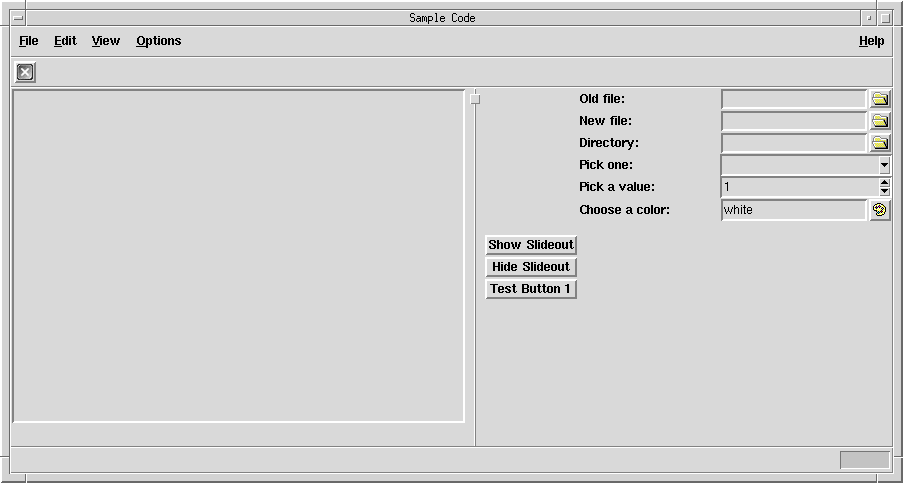
\includegraphics[width=5in]{MainWindow2.png}
\caption{Sample Main Window, slideout shown}
\label{fig:Main:MainWindow2}
\end{centering}
\end{figure}
Listing~\ref{lst:Main:MainWindowCode} contains code to create a basic
Main Window with a log window, simple set of command buttons, and a
slideout\footnote{See Chapter~\ref{chapt:LabelFrameWidgets} for the code used
to populate the slideout.}.  The window this code creates is shown in
Figures~\ref{fig:Main:MainWindow1} and \ref{fig:Main:MainWindow2}.

%* 
%* ------------------------------------------------------------------
%* LabelFrameWidgets.tex - Assorted LabelFrame widgets.
%* Created by Robert Heller on Thu Apr 19 14:39:49 2007
%* ------------------------------------------------------------------
%* Modification History: $Log$
%* Modification History: Revision 1.1  2007/05/06 12:49:38  heller
%* Modification History: Lock down  for 2.1.8 release candidate 1
%* Modification History:
%* Modification History: Revision 1.1  2002/07/28 14:03:50  heller
%* Modification History: Add it copyright notice headers
%* Modification History:
%* ------------------------------------------------------------------
%* Contents:
%* ------------------------------------------------------------------
%*  
%*     Model RR System, Version 2
%*     Copyright (C) 1994,1995,2002-2005  Robert Heller D/B/A Deepwoods Software
%* 			51 Locke Hill Road
%* 			Wendell, MA 01379-9728
%* 
%*     This program is free software; you can redistribute it and/or modify
%*     it under the terms of the GNU General Public License as published by
%*     the Free Software Foundation; either version 2 of the License, or
%*     (at your option) any later version.
%* 
%*     This program is distributed in the hope that it will be useful,
%*     but WITHOUT ANY WARRANTY; without even the implied warranty of
%*     MERCHANTABILITY or FITNESS FOR A PARTICULAR PURPOSE.  See the
%*     GNU General Public License for more details.
%* 
%*     You should have received a copy of the GNU General Public License
%*     along with this program; if not, write to the Free Software
%*     Foundation, Inc., 675 Mass Ave, Cambridge, MA 02139, USA.
%* 
%*  
%* 

\chapter{An Assortment of LabelFrame Based Widgets.}
\label{chapt:LabelFrameWidgets}
\typeout{$Id$}

\chapter{HTMLHelp}

\section{About}

The HTMLHelp widget is a help dialog that display program documentation
coded in a simple subset of HTML.  There is limited support for
Cascading Style Sheets.  There is a support for searching and there is a
simple history stack.

\section{Using the HTMLHelp widget}

The HTMLHelp is a SNIT widgetadaptor based on the BWidget Dialog widget.
It takes these options:

\begin{description}
\item[-textwidth] The width of the help text component (see -width of
the text widget).
\item[-width] The width of the HTMLHelp (see -width of the Dialog
widget).
\item[-height] The height of the HTMLHelp (see -height of the Dialog
widget).
\item[-side] The side to place the pane slider button.  Can be top (the
default) or bottom (see -side of the PanedWindow widget). This is a read
only option.
\item[-helpdirectory] The name of the directory where the HTML code
lives. This is a read only option.  There is no default value and this
option must be specified. (But see below for the typemethod
setDefaults.)
\item[-tableofcontents] The name of the HTML file in the help directory
that contains the Table Of Contents.  This is a read only option. 
There is no default value and this option must be specified. (But see
below for the typemethod setDefaults.)
\end{description}

There is one public method available:

\begin{verbatim}
$HTMLHelpObject helptopic topicstring
\end{verbatim}

This method searches the table of contents for a hyperlink with the
specified help topic string as the link text (case folded search) and
opens the HTMLHelp dialog with the page specified by the link
associated with this text.

There are two public typemethods available:

\begin{verbatim}
HTMLHelp::HTMLHelp setDefaults helpdir tocfile
\end{verbatim}

This method sets the default values for the \verb=-helpdirectory= and
\verb=-tableofcontents= options.

\begin{verbatim}
HTMLHelp::HTMLHelp help topicstring
\end{verbatim}

This typemethod just calls the \verb=helptopic= method for a default help
dialog object.  If a default help does not exist, it is created, using
the default values set by the \verb=setDefaults= typemethod.

\section{Creating Help text with \LaTeX\  and tex4ht}

Help text HTML files can be generated using \LaTeX\  and tex4ht.  You
need be sure you include a table of contents (\verb=\tableofcontents=)
and use the htlatex command with \verb=html,4,info= as its second
parameter. The former creates the index for the left column and the
latter breaks the file up into one file for each section.  Be sure to
include a chapter or section titled ``Help''\footnote{A sample chapter
is included with the development code as Help.tex.}, since this is used
as the topic text for the HTMLHelp dialog itself.  Generally you would
write a chapter, section or subsection for each help topic you expect
to have for your application -- that is for all of the Help buttons on
dialogs and Help menu items on main windows\footnote{See SampleCode.tex
for a sample documentation \LaTeX\  source file.}.





%* 
%* ------------------------------------------------------------------
%* CTCPanels.tex - Creating CTC Panels
%* Created by Robert Heller on Thu Apr 19 14:37:54 2007
%* ------------------------------------------------------------------
%* Modification History: $Log$
%* Modification History: Revision 1.2  2007/10/22 17:17:27  heller
%* Modification History: 10222007
%* Modification History:
%* Modification History: Revision 1.1  2007/05/06 12:49:38  heller
%* Modification History: Lock down  for 2.1.8 release candidate 1
%* Modification History:
%* Modification History: Revision 1.1  2002/07/28 14:03:50  heller
%* Modification History: Add it copyright notice headers
%* Modification History:
%* ------------------------------------------------------------------
%* Contents:
%* ------------------------------------------------------------------
%*  
%*     Model RR System, Version 2
%*     Copyright (C) 1994,1995,2002-2005  Robert Heller D/B/A Deepwoods Software
%* 			51 Locke Hill Road
%* 			Wendell, MA 01379-9728
%* 
%*     This program is free software; you can redistribute it and/or modify
%*     it under the terms of the GNU General Public License as published by
%*     the Free Software Foundation; either version 2 of the License, or
%*     (at your option) any later version.
%* 
%*     This program is distributed in the hope that it will be useful,
%*     but WITHOUT ANY WARRANTY; without even the implied warranty of
%*     MERCHANTABILITY or FITNESS FOR A PARTICULAR PURPOSE.  See the
%*     GNU General Public License for more details.
%* 
%*     You should have received a copy of the GNU General Public License
%*     along with this program; if not, write to the Free Software
%*     Foundation, Inc., 675 Mass Ave, Cambridge, MA 02139, USA.
%* 
%*  
%* 

\chapter{Creating CTC Panels}
\label{chapt:CTCPanels}
\typeout{$Id$}

Version 2 of the CTC Panel code is covered in this chapter.  Version 1
is depreciated and is included only for older applications.

\section{Creating a CTCPanel and creating objects to populate it.}
\begin{lstlisting}[caption={CTCPanel::CTCPanel procedure},
		   label={lst:CTC:CTCPanelproc}]
CTCPanel::CTCPanel widgetpath [options...]
\end{lstlisting}
CTCPanels are implemented with a Snit widget type and are created with
the CTCPanel::CTCPanel procedure, as shown in
Listing~\ref{lst:CTC:CTCPanelproc}. This widget takes four options:
\begin{description}
\item[-schematicbackground] The background color of the schematic
display. Defaults to black.
\item[-controlbackground] The background color of the control display.
Defaults to darkgreen.
\item[-width] The total width of the megawidget.
\item[-height] The total height of the megawidget.
\end{description}
\begin{lstlisting}[caption={CTCPanel::CTCPanel creating objects},
		   label={lst:CTC:CTCPanelcreate}]
$CTCPanelObject create type name [options...]
\end{lstlisting}
\begin{table}[hbpt]
\begin{centering}
\begin{tabular}{|l|p{3in}|}
\hline
Method & Description \\
\hline
\hline
getv & Gets the current value of the object.\\
\hline
setv & Set the value of the object.\\
\hline
geti & Gets the value of the specified indicator. \\
\hline
seti & Sets the value of the specified indicator. \\
\hline
itemcget & Gets the value of a specified option of the object.\\
\hline
itemconfigure & Sets the value of a specified option of the object.\\
\hline
exists & Tests to see of the object exists.\\
\hline
delete & Deletes the specified object.\\
\hline
move & Moves the specified object a relative distance.\\
\hline
class & Returns the class (or type) of the object.\\
\hline
invoke & Executes a script bound to an object.\\
\hline
coords & Returns the coordinates of a specified terminal element of the
object. \\
\hline
print & Writes a scriptlet to re-create the object to the specified
output stream.\\
\hline
\end{tabular}
\caption{Object methods}
\label{tab:CTC:ObjectMethods}
\end{centering}
\end{table}
The panel includes its own scrollbars, including a shared horizontal
scrollbar. Items displayed on the CTCPanel (either as schematic
trackwork in the schematic display or as control items in the control
display) are created with the create command, as shown in
Listing~\ref{lst:CTC:CTCPanelcreate}.  Each object has a unique name, a
value, zero or more indicators, and zero or more options.  The CTCPanel
widget defines thirteen methods that take an object name, as shown in
Table~\ref{tab:CTC:ObjectMethods}. 

\section{Control Points}

Objects on a CTCPanel are grouped into named Control Points.  A Control
Point defines one (or more) trackwork elements and their corresponding
control panel elements.  In the simplest case a control point might
include a Switch (turnout), a SIGPlate, a SWPlate, and a CodeButton,
with the SWPlate controlling the Switch and the SIGPlate controlling the
signals surrounding the Switch.

\section{Object values and invocation}

Many objects have an associated value.  Generally, these values
represent state information and these values (or states) correspond to
different scripts bound to the object.  For example trackwork switches
(turnouts) define their state as being normal (points aligned for the
main line) or reversed (points aligned for the branch line).

Also many objects have \lstinline=-command= options, which define
scriptlets to invoke under certain conditions.  One (or more) of these
scriptlets are executed (at the global level) when the object is
invoked.  Generally, trackwork objects are invoked to acquire state
information (such as occupancy or point state feedback) from input
ports bits (such as read from a Chubb CMR/I serial bus), and control
objects are invoked to read and effect control panel settings by
setting output port bits for trackwork control and signals.  Generally,
the \lstinline=-command= bound to a code button will in turn invoke all
of the objects associated with the control point the code button
manages.

All trackwork objects have an \lstinline=-occupiedcommand= option,
which is a script to run to fetch the object's occupied state.  The
invoke method always returns the occupied state (always false for
objects that are not trackwork objects).  Trackwork with movable points
should not have their points moved which a train is occupying the
trackwork!  Generally, if any of the trackwork of a control point is
occupied, the control point's code button should not invoke any of the
control elements.

\section{Sample CTCPanel and the code to create it.}

\lstinputlisting[caption={Creating a CTC Panel},
		 label={lst:CTC:CTCPanelCode},
		 firstline=36]{SampleCodeCTCPanel.tcl}
\begin{figure}[hbpt]
\begin{centering}
\includegraphics{CTCPanel.png}
\caption{Sample CTC Panel Screen Shot}
\label{fig:CTC:CTCPanelWindow}
\end{centering}
\end{figure}
The Tcl  code in Listing~\ref{lst:CTC:CTCPanelCode} creates a simple
CTC Panel\footnote{See~\cite{tclinternals}, Section 1.4 for a complete
list of available panel elements.}. The CTC Panel itself is created at
line 61 Lines 67--192 populate the panel with both control panel
elements and track schematic elements.  The panel is shown in
Figure~\ref{fig:CTC:CTCPanelWindow}.  

This CTC Panel features a switch (turnout) off the main line to an
industrial spur. There is one actual control point, named SP1, and
three blocks, two for the mainline blocks and one for the industrial
spur.  I have put each block into a separate logical control point as a
organizational  convenience.  The control point SP1 contains one piece
of trackwork, the switch, and four control panel items, a switch plate,
a signal plate, a code button, and a label.  The code does not interact
with an actual layout.  Normally, the \lstinline=-occupiedcommand= 
options of the trackwork elements would define code to read block
occupancy detectors and the \lstinline=-statecommand= of the switch
would define code to read the switch's point position feedback
sensors\footnote{Using the  CMR/I (Bruce Chubb) Interface, as described
in Chapter~\ref{chapt:CMRI:CMRIProgramming}, for example.}. The code
for the switch plate (procedure SetSwitchSP1) would just set the output
bits to activate the switch's switch machine.  The signal plate code
(procedure SetSignalSP1) would also set the output bits to update the
aspects of the signals protecting the switch.


%* 
%* ------------------------------------------------------------------
%* ReadConfiguration.tex - Reading Configuration files
%* Created by Robert Heller on Thu Apr 19 14:44:47 2007
%* ------------------------------------------------------------------
%* Modification History: $Log$
%* Modification History: Revision 1.2  2007/10/22 17:17:27  heller
%* Modification History: 10222007
%* Modification History:
%* Modification History: Revision 1.1  2007/05/06 12:49:39  heller
%* Modification History: Lock down  for 2.1.8 release candidate 1
%* Modification History:
%* Modification History: Revision 1.1  2002/07/28 14:03:50  heller
%* Modification History: Add it copyright notice headers
%* Modification History:
%* ------------------------------------------------------------------
%* Contents:
%* ------------------------------------------------------------------
%*  
%*     Model RR System, Version 2
%*     Copyright (C) 1994,1995,2002-2005  Robert Heller D/B/A Deepwoods Software
%* 			51 Locke Hill Road
%* 			Wendell, MA 01379-9728
%* 
%*     This program is free software; you can redistribute it and/or modify
%*     it under the terms of the GNU General Public License as published by
%*     the Free Software Foundation; either version 2 of the License, or
%*     (at your option) any later version.
%* 
%*     This program is distributed in the hope that it will be useful,
%*     but WITHOUT ANY WARRANTY; without even the implied warranty of
%*     MERCHANTABILITY or FITNESS FOR A PARTICULAR PURPOSE.  See the
%*     GNU General Public License for more details.
%* 
%*     You should have received a copy of the GNU General Public License
%*     along with this program; if not, write to the Free Software
%*     Foundation, Inc., 675 Mass Ave, Cambridge, MA 02139, USA.
%* 
%*  
%* 

\chapter{Managing preferences or configuration options}
\label{chapt:ReadConfiguration}
\typeout{$Id$}

The ReadConfiguration package provides functions for reading, writing,
and editing preferences or configuration options.  The procedure
\lstinline=ReadConfiguration::ReadConfiguration= reads in a
configuration or preferences file. The
\lstinline=ReadConfiguration::WriteConfiguration= procedure writes a
configuration or preferences file. and the snit macro
\lstinline=ReadConfiguration::ConfigurationType= creates a snit type to
hold a set of configuration options or preferences.

\section{Configuration or preferences files}

Each logical line can contain either an unnamed value (an anonoymous
configuration option) or a name value pair.  The value can be either a
scalar value or a brace enclosed list of alternating keys and values.
Tcl bracing, quoting, and comment conventions are used in this file.

Both \lstinline=ReadConfiguration::ReadConfiguration= and
\lstinline=ReadConfiguration::WriteConfiguration= take the same two
arguments--a filename and the name of an array variable to receive or
provide the preferences.

\section{A complete Snit type object to hold and manage preferences}

\lstinputlisting[caption={Creating a configuration object},
		 label={lst:RC:ConfigurationType},
		 firstline=36]{SampleCodeRC.tcl}
\begin{figure}[hbpt]
\begin{centering}   
\includegraphics{EditConf.png}
\caption{Editing a set of preferences}
\label{fig:RC:EditConf}
\end{centering}
\end{figure}
The macro \lstinline=ReadConfiguration::ConfigurationType= can be used
to create an ensemble command to hold the preferences or configuration
options for your program.  This macro generates a Snit type that include
type methods to load, save, edit, and access preference or configuration
options. Typical code to use this macro is shown in
Listing~\ref{lst:RC:ConfigurationType} and the dialog box this macro
generates is shown in Figure~\ref{fig:RC:EditConf}.


%* 
%* ------------------------------------------------------------------
%* GraphicsSupport.tex - Using the graphics support code.
%* Created by Robert Heller on Thu Apr 19 14:38:52 2007
%* ------------------------------------------------------------------
%* Modification History: $Log$
%* Modification History: Revision 1.1  2007/05/06 12:49:38  heller
%* Modification History: Lock down  for 2.1.8 release candidate 1
%* Modification History:
%* Modification History: Revision 1.1  2002/07/28 14:03:50  heller
%* Modification History: Add it copyright notice headers
%* Modification History:
%* ------------------------------------------------------------------
%* Contents:
%* ------------------------------------------------------------------
%*  
%*     Model RR System, Version 2
%*     Copyright (C) 1994,1995,2002-2005  Robert Heller D/B/A Deepwoods Software
%* 			51 Locke Hill Road
%* 			Wendell, MA 01379-9728
%* 
%*     This program is free software; you can redistribute it and/or modify
%*     it under the terms of the GNU General Public License as published by
%*     the Free Software Foundation; either version 2 of the License, or
%*     (at your option) any later version.
%* 
%*     This program is distributed in the hope that it will be useful,
%*     but WITHOUT ANY WARRANTY; without even the implied warranty of
%*     MERCHANTABILITY or FITNESS FOR A PARTICULAR PURPOSE.  See the
%*     GNU General Public License for more details.
%* 
%*     You should have received a copy of the GNU General Public License
%*     along with this program; if not, write to the Free Software
%*     Foundation, Inc., 675 Mass Ave, Cambridge, MA 02139, USA.
%* 
%*  
%* 

\chapter{Using the Graphics Support Code.}
\label{chapt:GraphicsSupport}
\typeout{$Id}


%* 
%* ------------------------------------------------------------------
%* PanelInstruments.tex - Using the Panel Instruments Widgets
%* Created by Robert Heller on Thu Apr 19 14:43:50 2007
%* ------------------------------------------------------------------
%* Modification History: $Log$
%* Modification History: Revision 1.2  2007/11/30 13:56:50  heller
%* Modification History: Novemeber 30, 2007 lockdown.
%* Modification History:
%* Modification History: Revision 1.1  2007/05/06 12:49:39  heller
%* Modification History: Lock down  for 2.1.8 release candidate 1
%* Modification History:
%* Modification History: Revision 1.1  2002/07/28 14:03:50  heller
%* Modification History: Add it copyright notice headers
%* Modification History:
%* ------------------------------------------------------------------
%* Contents:
%* ------------------------------------------------------------------
%*  
%*     Model RR System, Version 2
%*     Copyright (C) 1994,1995,2002-2005  Robert Heller D/B/A Deepwoods Software
%* 			51 Locke Hill Road
%* 			Wendell, MA 01379-9728
%* 
%*     This program is free software; you can redistribute it and/or modify
%*     it under the terms of the GNU General Public License as published by
%*     the Free Software Foundation; either version 2 of the License, or
%*     (at your option) any later version.
%* 
%*     This program is distributed in the hope that it will be useful,
%*     but WITHOUT ANY WARRANTY; without even the implied warranty of
%*     MERCHANTABILITY or FITNESS FOR A PARTICULAR PURPOSE.  See the
%*     GNU General Public License for more details.
%* 
%*     You should have received a copy of the GNU General Public License
%*     along with this program; if not, write to the Free Software
%*     Foundation, Inc., 675 Mass Ave, Cambridge, MA 02139, USA.
%* 
%*  
%* 

\chapter{Using the Panel Instruments Widgets}
\label{chapt:PanelInstruments}
\typeout{$Id$}
\lstinputlisting[caption={Using the Panel Instrument based widgets},
		 label={lst:PI:SampleCodeInstrumentPanel},
		 firstline=38]{SampleCodeInstrumentPanel.tcl}
\begin{figure}[hbpt]
\begin{centering}
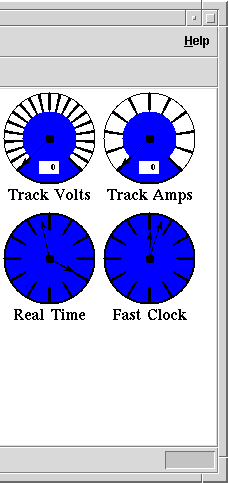
\includegraphics{PanelInstrument.png}
\caption{Some Panel Instruments}
\label{fig:PI:PanelInstrument}
\end{centering}
\end{figure}
Listing~\ref{lst:PI:SampleCodeInstrumentPanel} contains code to create
some of the panel instrument widgets.  The window this code helped to
create is shown in Figure~\ref{fig:PI:PanelInstrument}. Several typical
panel instruments are shown with the code to create them.


%* 
%* ------------------------------------------------------------------
%* OvalWidgets.tex - Oval Widgets
%* Created by Robert Heller on Thu Apr 19 14:42:53 2007
%* ------------------------------------------------------------------
%* Modification History: $Log$
%* Modification History: Revision 1.1  2007/05/06 12:49:38  heller
%* Modification History: Lock down  for 2.1.8 release candidate 1
%* Modification History:
%* Modification History: Revision 1.1  2002/07/28 14:03:50  heller
%* Modification History: Add it copyright notice headers
%* Modification History:
%* ------------------------------------------------------------------
%* Contents:
%* ------------------------------------------------------------------
%*  
%*     Model RR System, Version 2
%*     Copyright (C) 1994,1995,2002-2005  Robert Heller D/B/A Deepwoods Software
%* 			51 Locke Hill Road
%* 			Wendell, MA 01379-9728
%* 
%*     This program is free software; you can redistribute it and/or modify
%*     it under the terms of the GNU General Public License as published by
%*     the Free Software Foundation; either version 2 of the License, or
%*     (at your option) any later version.
%* 
%*     This program is distributed in the hope that it will be useful,
%*     but WITHOUT ANY WARRANTY; without even the implied warranty of
%*     MERCHANTABILITY or FITNESS FOR A PARTICULAR PURPOSE.  See the
%*     GNU General Public License for more details.
%* 
%*     You should have received a copy of the GNU General Public License
%*     along with this program; if not, write to the Free Software
%*     Foundation, Inc., 675 Mass Ave, Cambridge, MA 02139, USA.
%* 
%*  
%* 

\chapter{Using the Oval Widgets}
\label{chapt:OvalWidgets}
\typeout{$Id$}


%* 
%* ------------------------------------------------------------------
%* LCARSWidgets.tex - LCARS Widgets
%* Created by Robert Heller on Thu Apr 19 14:40:59 2007
%* ------------------------------------------------------------------
%* Modification History: $Log$
%* Modification History: Revision 1.1  2007/05/06 12:49:38  heller
%* Modification History: Lock down  for 2.1.8 release candidate 1
%* Modification History:
%* Modification History: Revision 1.1  2002/07/28 14:03:50  heller
%* Modification History: Add it copyright notice headers
%* Modification History:
%* ------------------------------------------------------------------
%* Contents:
%* ------------------------------------------------------------------
%*  
%*     Model RR System, Version 2
%*     Copyright (C) 1994,1995,2002-2005  Robert Heller D/B/A Deepwoods Software
%* 			51 Locke Hill Road
%* 			Wendell, MA 01379-9728
%* 
%*     This program is free software; you can redistribute it and/or modify
%*     it under the terms of the GNU General Public License as published by
%*     the Free Software Foundation; either version 2 of the License, or
%*     (at your option) any later version.
%* 
%*     This program is distributed in the hope that it will be useful,
%*     but WITHOUT ANY WARRANTY; without even the implied warranty of
%*     MERCHANTABILITY or FITNESS FOR A PARTICULAR PURPOSE.  See the
%*     GNU General Public License for more details.
%* 
%*     You should have received a copy of the GNU General Public License
%*     along with this program; if not, write to the Free Software
%*     Foundation, Inc., 675 Mass Ave, Cambridge, MA 02139, USA.
%* 
%*  
%* 

\chapter{Various LCARS Widgets}
\label{chapt:LCARSWidgets}
\typeout{$Id$}

%* 
%* ------------------------------------------------------------------
%* StarKitsStarPacks.tex - Creating StarKits and StarPacks
%* Created by Robert Heller on Thu Apr 19 14:46:59 2007
%* ------------------------------------------------------------------
%* Modification History: $Log$
%* Modification History: Revision 1.1  2007/05/06 12:49:39  heller
%* Modification History: Lock down  for 2.1.8 release candidate 1
%* Modification History:
%* Modification History: Revision 1.1  2002/07/28 14:03:50  heller
%* Modification History: Add it copyright notice headers
%* Modification History:
%* ------------------------------------------------------------------
%* Contents:
%* ------------------------------------------------------------------
%*  
%*     Model RR System, Version 2
%*     Copyright (C) 1994,1995,2002-2005  Robert Heller D/B/A Deepwoods Software
%* 			51 Locke Hill Road
%* 			Wendell, MA 01379-9728
%* 
%*     This program is free software; you can redistribute it and/or modify
%*     it under the terms of the GNU General Public License as published by
%*     the Free Software Foundation; either version 2 of the License, or
%*     (at your option) any later version.
%* 
%*     This program is distributed in the hope that it will be useful,
%*     but WITHOUT ANY WARRANTY; without even the implied warranty of
%*     MERCHANTABILITY or FITNESS FOR A PARTICULAR PURPOSE.  See the
%*     GNU General Public License for more details.
%* 
%*     You should have received a copy of the GNU General Public License
%*     along with this program; if not, write to the Free Software
%*     Foundation, Inc., 675 Mass Ave, Cambridge, MA 02139, USA.
%* 
%*  
%* 

\chapter{Creating StarKits and StarPacks}
\label{chapt:StarKitsStarPacks}
\typeout{$Id$}


\lstinputlisting[caption={Makefile fragment for building a StarPack},
		 label={lst:STR:Makefile},
		 firstline=152,lastline=174]{Makefile.am}
The Makefile fragment shown in Listing~\ref{lst:STR:Makefile} builds a
StarPack.  It starts by removing any existing kit or kit
directory\footnote{Basicly, cleaning up from a previously failed
build.}. Then it uses the SDX qwrap and unwrap commands to create a base
level kit directory.  It then uses helper kits to populate this
directory with additional scripts and data files, then finally wraps the
resulting directory into a StarPack with the SDX wrap command (the
\lstinline=-runtime= option makes this a StarPack rather than a
StarKit).

\section{Helper programs included with the Model Railroad System}

Three tclkits are included with the Model Railroad System to help you
build your own programs using elements of the Model Railroad System
Tcl/Tk library of packages:
\begin{description}
\item[AddKitDir.kit] This kit adds a symbolic link to a directory in a
kit directory tree.  This is a ``lazy'' copy of a directory that is usually a
directory containing a Tcl/Tk package.
\item[AddKitFile.kit] This kit adds one or more files to a directory in
a kit directory tree.
\item[MakePkgIndex.kit] This kit runs the Tcl command
\lstinline=pkg_mkIndex= on a directory under the lib directory in a kit
directory tree.
\end{description}
These tclkits help with some of the common tasks involved in build
StarKits and StarPacks.

\subsection{AddKitDir.kit -- Add a directory to a StarKit or StarPack}

This kit does a ``lazy'' copy\footnote{Simply a symbolic link.} of a
directory to a StarKit's or StarPack's vfs\footnote{Virtual File System.}
directory.  It takes three parameters: the name of the kit (without the
\lstinline=.kit= or \lstinline=.vfs= extension), the relative path to
the parent directory, and the path to the directory to add.  A symbolic link,
using the tail of the directory path to add, is made in the StarKit's or
StarPack's \lstinline=.vfs= directory under the relative path specified.

\begin{lstlisting}[label={lst:STR:addkitdir},caption={Adding a directory
to a kit.}]
tclkit AddKitDir.kit MyProgram lib /usr/share/bwidget1.8.0
\end{lstlisting}

The example in Listing~\ref{lst:STR:addkitdir} adds a symbolic link
named \lstinline=bwidget1.8.0= to \lstinline=/usr/share/bwidget1.8.0= in
\lstinline=MyProgram.vfs/lib/=. When the kit is wrapped, the sdx program
will make a deep copy of this directory into the resultant kit or pack.

\subsection{AddKitFile.kit -- Add files to a StarKit or StarPack}

This kit copies one or more files to a directory in
a StarKit's or StarPack's vfs directory. It takes three or more
parameters: the name of the kit (without the \lstinline=.kit= or
\lstinline=.vfs= extension), the relative path to directory to add files
to\footnote{The directory is created if it does not already exist.}, and
one or more files to copy.

\begin{lstlisting}[label={lst:STR:addkitfile},caption={Adding files to a
 kit.}]
tclkit AddKitFile.kit MyProgram lib/packages mypackage1.tcl \
			mypackage2.tcl myextension.so 
\end{lstlisting}

The example in Listing~\ref{lst:STR:addkitfile} adds the files
\lstinline=mypackage1.tcl=, \lstinline=mypackage2.tcl=, and
\lstinline=myextension.so= to the directory
\lstinline=MyProgram.vfs/lib/packages=. 

\subsection{MakePkgIndex.kit -- Create a pkgIndex.tcl file for a
directory in a StarKit or StarPack}

This kit runs \lstinline=pkg_mkIndex= on a directory under the
\lstinline=lib= directory in a StarKit's or StarPack's vfs directory. It
takes two parameters: the name of the kit (without the \lstinline=.kit=
or \lstinline=.vfs= extension) and the directory under the
\lstinline=lib= directory to run \lstinline=pkg_mkIndex= over.

\begin{lstlisting}[label={lst:STR:makepkgindex},caption={Creating the
pkgIndex.tcl for a directory of packages in a kit.}]
tclkit MakePkgIndex.kit MyProgram packages
\end{lstlisting}

The example in Listing~\ref{lst:STR:makepkgindex} runs 
\lstinline=pkg_mkIndex= over the directory
\lstinline=MyProgram.vfs/lib/packages=. 


%
\cleardoublepage
\bibliography{MRR}
\bibliographystyle{plain}
\cleardoublepage
\printindex
\end{document}



